\documentclass{beamer}
\usepackage[spanish]{babel}
\selectlanguage{spanish}
\usepackage[utf8]{inputenc}
\usepackage{hyperref}
\usepackage{graphicx}
\usepackage{float}


\usetheme{Frankfurt}
\usecolortheme{whale}

\title{Merges}
\author{Emmanuel Arias \href{mailto:emmanuelarias30@gmail.com}{emmanuelarias30@gmail.com}}
\date{}
\begin{document}
\begin{frame}[plain]
    \maketitle
\end{frame}

\begin{frame}{git merge}
	\begin{itemize}
		 \item El comando \textit{git merge} te permite tomar las líneas de desarrollo independientes creadas por \textit{git branch} e integrarlas en una sola rama.
		 \item Todos los comandos que veremos hacen fusionar en la rama actual. 
		 \item La rama actual se actualizará para reflejar la fusión, pero la rama de destino no se verá afectada por completo.¸
	\end{itemize}
\end{frame}

\begin{frame}{Merge}
\begin{figure}
	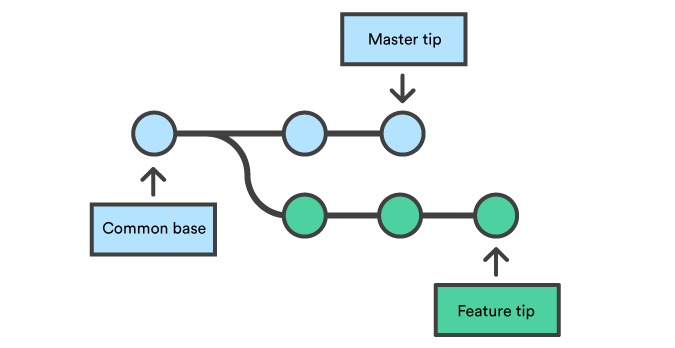
\includegraphics[width=1\linewidth]{img/Branch-2}
	\label{fig:branch-2}
\end{figure}
\end{frame}

\begin{frame}{Merge}
	\begin{figure}
		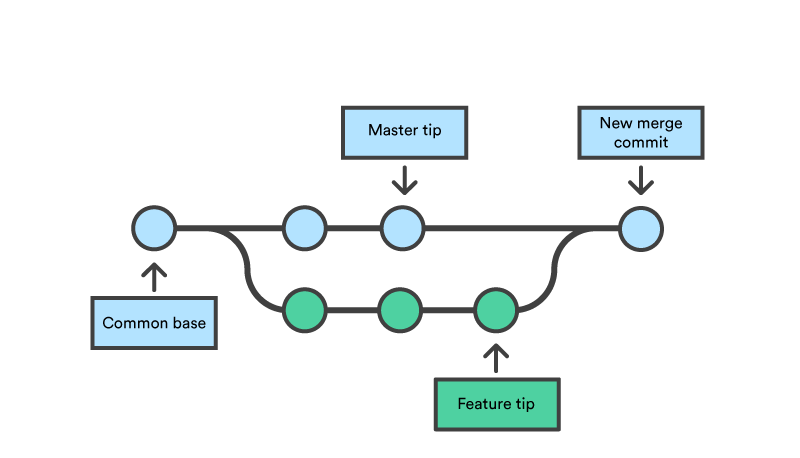
\includegraphics[width=1\linewidth]{img/Branch-3}
		\label{fig:branch-3}
	\end{figure}
\end{frame}


\begin{frame}{Prepararnos para el merge}
\begin{itemize}
	\item Primer asegurarnos dónde estamos parados. Ejecutar \textit{git status} para asegurarnos que HEAD está apuntando
	correctamente a la rama que va a recibir el merge.
	\item Actualizar la rama dónde voy a mergear.
	\item Mergear
\end{itemize}
\end{frame}

\begin{frame}{}
	\center\Huge{Fast Forward Merge}
\end{frame}

\begin{frame}{Fast Forward Merge}
\begin{figure}
	\centering
	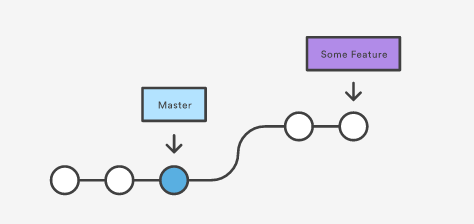
\includegraphics[width=1\linewidth]{1}
	\label{fig:1}
\end{figure}
\end{frame}

\begin{frame}{Fast Forward Merge}
	\begin{figure}
		\centering
		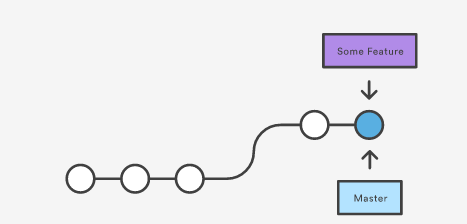
\includegraphics[width=1\linewidth]{2}
		\label{fig:2}
	\end{figure}
\end{frame}


\begin{frame}{}
	\center\Huge{3-way merge}
\end{frame}


\begin{frame}{3-way merge}
\begin{figure}
	\centering
	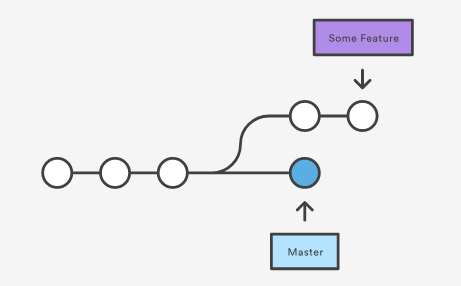
\includegraphics[width=1\linewidth]{3}
	\label{fig:3}
\end{figure}
\end{frame}

\begin{frame}{3-way merge}
\begin{figure}
	\centering
	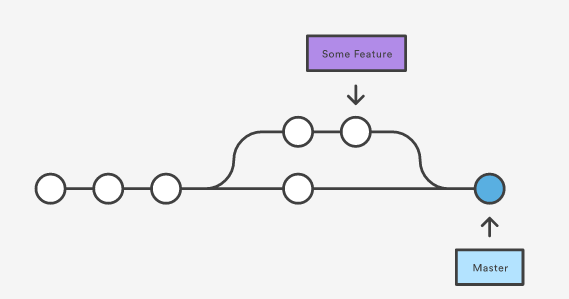
\includegraphics[width=1\linewidth]{4}
	\label{fig:4}
\end{figure}
\end{frame}

\begin{frame}{}
	\center\Huge{Resolviendo el conflictos}
\end{frame}

\begin{frame}{}
	\center\Huge{Rebase}
\end{frame}


\end{document}
